\documentclass[a4paper,11pt]{article}
\usepackage[T1]{fontenc}
\usepackage[utf8]{inputenc}
\usepackage{lmodern}
\usepackage{graphicx}

\newcommand{\documentTitle}{A DAG of components -- for an internal architecture too}
\author{Sébastien \textsc{Wilmet}}
\date{January 15, 2020}

\title{\documentTitle}

% Page margins
%\usepackage[top=2cm, bottom=3cm, left=2.5cm, right=2.5cm]{geometry}

% PDF file properties and links
\usepackage{hyperref}
\hypersetup{
  pdfauthor   = {Sébastien Wilmet},
  pdftitle    = {\documentTitle},
  pdfcreator  = {TeX Live},
  pdfproducer = {TeX Live},
  colorlinks  = false,
  pdfborder   = 0 0 0
}

\begin{document}

\maketitle
\tableofcontents

% \bigskip

% Replaced by the introduction.
% \begin{abstract}
%   After a general introduction, this article deals with the topic of integrating several software modules together -- for example a set of libraries plus an application. In other words, what we call a software stack, but is actually a directed acyclic graph (DAG). Then the discussion zooms in to focus on a \emph{single} module, and some benefits of having a DAG as the internal architecture of a module.
% \end{abstract}

\pagebreak

\section{Introduction -- a DAG of components}

\begin{figure}
  \begin{center}
    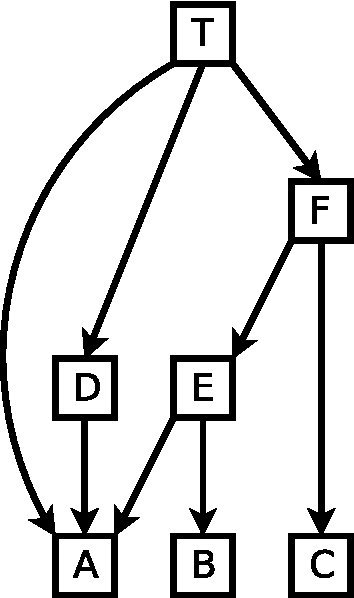
\includegraphics[scale=0.5]{images/dag.pdf}
    \caption{A directed acyclic graph (DAG) of software components.}
    \label{fig:dag}
  \end{center}
\end{figure}

Figure~\ref{fig:dag} shows a directed acyclic graph (DAG) of software components. The letter T at the top is --~well now you've guessed it~-- for the Top of the graph.

In this article we use \emph{component} as a general term to designate both:
\begin{itemize}
  \item A software \emph{module} (for example a library or an application).
  \item A \emph{class}, in the internal architecture of a module, supposing that the module follows an Object-Oriented Programming (OOP) paradigm.
\end{itemize}

This article begins with a DAG of modules (section~\ref{dag-of-modules}), to integrate several modules together. It explains why it's a DAG. We will also see that when integrating several modules together, it is better to do it \emph{gradually}, not by trying to build and test all the modules at once.

Then the section~\ref{dag-of-classes} explains why it is a good idea to have a DAG of classes as the internal architecture of a module. With several possible applications: being able to better test internal classes (either with unit tests or interactive tests), and porting a module gradually to a new major version of an underlying library that breaks its API in an inconvenient way.

\section{A DAG of modules}
\label{dag-of-modules}

This section deals with the topic of integrating several software modules together -- for example a set of libraries plus an application. In other words, what we call a software stack, but is actually a directed acyclic graph (DAG).

Note that we are not advocating for using the ``software DAG'' terminology in everyday conversations, ``software stack'' is fine, but knowing that it's a DAG can help when reasoning about the system.

\subsection{It's directed, ideally acyclic, and it's a graph}
When an application uses a library, it has a \emph{use} relationship with that library. Likewise, a library may use a lower-level library, and so on, and other software components may be used as well, such as a database system, daemons, etc, until we reach the operating system kernel. But we can go beyond the software/hardware boundary, and arguably the kernel in turn uses the computer hardware, which ultimately relies on the laws of science that govern our Universe, the Big Bang and (maybe) beyond. But I digress.

So, with the \emph{use} relationship, we've just explained the ``directed'' term of ``directed acyclic graph''. The relationship has a direction, the application \emph{uses} a library. To give an example, in Figure~\ref{fig:dag} p.~\pageref{fig:dag}, the module~T is the application, the module~D is a library, and the module~A is a lower-level library.

In a general setting it's a graph, not a stack or a tree, because low-level libraries can be used by both a higher-level library \emph{and} the application.

And now the last term of ``directed acyclic graph'' not yet explained: ``acyclic''. If there is a cycle in the graph, the use relationship goes in the two directions; for example an application uses a library and the library uses the application, or more probably two libraries use each other. While a cycle is sometimes unavoidable for certain low-level components such as a compiler that needs to use itself to compile its own source code, it is better to avoid cycles like this. When there is a cycle, it is painful to integrate the modules (which one to build first?), so a bootstrap phase is necessary or other tricks are used, such as copying the source code of one module into the other.

The Top of the graph is an end-user software, an application. The underlying software components is like the hidden part of an iceberg, the end-user is unaware of it, but in terms of lines of code it makes the bulk of the work.

Another example of a DAG of components is Unix command line utilities and shell pipes or scripts. When we re-use a lot of components to build a new program, it's like standing on shoulders of giants (especially when we talk about Unix, one can say).

\subsection{Gradually integrating several modules together}
\label{integration}

What the venerable book \emph{The Mythical Man-Month}\footnote{
Frederick P. \textsc{Brooks}, Jr.,
\emph{The Mythical Man-Month --- Essays on Software Engineering},
Anniversary Edition, Addison-Wesley, 1995.
} teaches us, among other things, is that for integrating several modules together (by supposing that each module has already been tested individually), it should be done by adding one component at a time and writing integration tests (chapter~13, ``The Whole and the Parts''), not by doing everything at once:

\begin{quotation}
  ``\textbf{Add one component at a time.}\hspace{0.5cm} This precept, too, is obvious, but optimism and laziness tempt us to violate it. To do it requires dummies and other scaffolding, and that takes work. And after all, perhaps all that work won't be needed? Perhaps there are no bugs?

  No! Resist the temptation! That is what systematic system testing is all about. One must assume that there will be lots of bugs, and plan an orderly procedure for snaking them out.

  Note that one must have thorough test cases, testing the partial systems after each new piece is added. And the old ones, run successfully on the last partial sum, must be rerun on the new one to test for system regression.''
\end{quotation}

\section{A DAG of classes as an internal architecture}
\label{dag-of-classes}

We now zoom in to look \emph{inside} a module, supposing that it is implemented with the Object-Oriented Programming paradigm.

In OOP, one component of the graph can be seen as one class. The edges of the graph represent class relationships, when a class depends on another, either via composition or via inheritance. So it is also a \emph{directed} graph. The central question is: why is it a good thing to have no cycles in such a graph? In other words, to have a DAG?

The same Figure~\ref{fig:dag} (still on p.~\pageref{fig:dag}) can be used as a reference. Each component is now (roughly) a class. In an application, there is a single entry point (in C it's the \texttt{main()} function), which corresponds to the Top of the graph. On the other hand a library may have several entry points, for example a toolkit providing independent utility classes will have several top-level nodes in the graph.

\subsection{The result of applying OOP best-practices}

To answer the question about why a DAG of classes is better for the internal architecture of a module: it stems from applying several OOP best-practices described in \emph{Object-Oriented Design Heuristics}\footnote{
Arthur \textsc{Riel},
\emph{Object-Oriented Design Heuristics},
Addison-Wesley, 1996.
}. This section builds upon these OOP best-practices, to go beyond what the book covers, and tries to innovate (without knowing if somebody else has come up to our same conclusion, and without knowing if an article has already been published about it).

\subsubsection{Composition -- a DAG for the containment hierarchy}
\label{dag-of-classes--composition}

First, if one class depends on another via \emph{composition}, here is the relevant OOP best-practice:
\begin{quotation}
  ``Heuristic 4.13: A class must know what it contains, but it should never know who contains it.''
\end{quotation}

If this heuristic is violated, then the relationship between the two classes goes in the two directions, and there is a cycle in the graph: the container has a reference to the child object, and the child object has a reference to the container.

If the heuristic is followed for all the containment hierarchy, then it forms a DAG. It permits to have more re-usable code. For instance the leaf classes are self-contained and can thus be copied to another project directly.

\begin{figure}[p]
  \begin{center}
    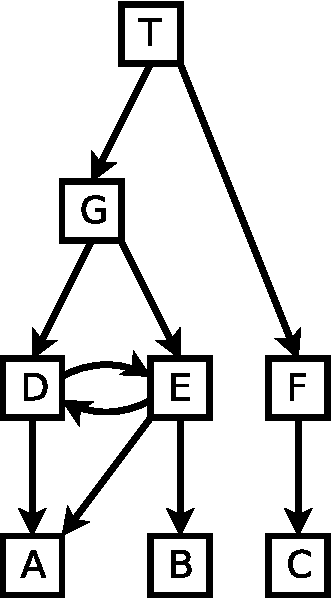
\includegraphics[scale=0.5]{images/graph-with-localized-cycle.pdf}
    \caption{Example of a containment hierarchy for the internal architecture of a module. A directed graph with a localized cycle -- sometimes unavoidable.}
    \label{fig:graph-with-localized-cycle}
  \end{center}
\end{figure}

However, there are situations where a cycle \emph{is} necessary, for example for performance reasons. In that case, it is better to keep the cycle in the graph as localized as possible, as in Figure~\ref{fig:graph-with-localized-cycle} p.~\pageref{fig:graph-with-localized-cycle}.

\begin{figure}[p]
  \begin{center}
    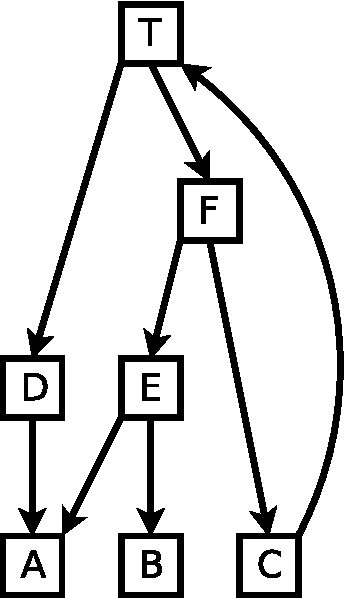
\includegraphics[scale=0.5]{images/graph-with-bad-cycle.pdf}
    \caption{Example of a containment hierarchy for the internal architecture of a module. A directed graph with a cycle that should be avoided -- \textbf{bad} example.}
    \label{fig:graph-with-bad-cycle}
  \end{center}
\end{figure}

A bad example is when a leaf class has access to the top-level class somehow, it means that it has access to the whole graph if there are public methods to get the objects (see Figure~\ref{fig:graph-with-bad-cycle} p.~\pageref{fig:graph-with-bad-cycle}). So, a ``leaf'' class could possibly depend on any other class of the module, which creates tight-coupling and spaghetti code. This should be avoided.

With a DAG, it's a cleaner architecture. Instead of having everything mixed together, features are built on top of more elementary features. If the codebase is well documented, with the possibility to browse the API documentation outside of the source code, then just reading the API documentation by following a bottom-up approach is a convenient way for a newcomer to get accustomed with the codebase.

\subsubsection{Inheritance}

For class inheritance, the OOP best-practice that interests us is:
\begin{quotation}
  ``Heuristic 5.2: Derived classes must have knowledge of their base class by definition, but base classes should not know anything about their derived classes.''
\end{quotation}

When this guideline is violated, the base class typically checks the type of the \emph{self} object to execute different instructions depending on which subclass it is. This of course should be avoided, it is better to use polymorphism instead.

As a result, an inheritance hierarchy forms a tree\footnote{And a tree is a DAG. But a DAG is not necessarily a tree.}, or a DAG if multiple inheritance is allowed.

\subsubsection{Generalization}

When we take into account both composition and inheritance, plus other types of dependencies like calling a static method of another class, it creates a dependency graph between the different classes or source files. When the resulting graph is a tree, a DAG, or a graph with only localized cycles, then it brings several benefits that we believe are important for a software project that is maintained in the long run.

As already discussed in section~\ref{dag-of-classes--composition}, it brings a clearer code structure, and more code re-usability. And it is possible to apply what is described in the next two sections. Read on!

\subsection{Testing of classes in a DAG}
\label{dag-testing}

For the sake of argument, let's take a GUI application as example of a module.

If all the code is entangled, when there is tight-coupling between lots of classes, then it's difficult to take one class and test it, since by taking that class you need to take basically all the rest of the application as well. The only interactive test that you can do is to launch the whole application. And when writing automated tests for graphical components, the tests need to also be run against the whole application.

On the other hand, with a DAG as the code structure, it's possible to take a subset of the DAG (choosing one class and following the edges until reaching the leaf classes) and test that subset independently. By doing this it's easier to write unit tests. It's possible to stress-test a component, to trigger all possible situations more easily.

For example with a widget that shows an error in the case where there is no more room on the filesystem, with buttons for different actions, we would like to test if the widget is shown correctly. With a DAG, it's possible to write a mini-application that just displays that widget regardless of whether the filesystem is full. That mini-application can serve as an interactive test, but it can also be used to write an automated test to ensure that there are no runtime warnings or errors when showing the widget, and that the buttons are in the right order (for example). It would be more difficult to test the same by launching the real application.

If the codebase has no unit tests, a strategy is to first start by writing tests for the leaf classes, to ensure that the foundations are solid, and then following a bottom-up approach, to walk up the DAG and write tests for higher-level components. Until reaching the top-level component, for which the tests can be called ``end-to-end tests''. This is a bit related to the section~\ref{integration} where we saw how to properly integrate several modules together, by doing it gradually.

\subsection{Build system support to have a smooth repercussion of an API break}

When a library breaks its API, it is often painful for users of that library. Ideally a new major version of a library just gets rid of API that has been deprecated in the previous major version, with replacements being available also in the previous version. But that is not always the case, sometimes a library changes the API during the development of the new major version, and the new APIs are not available in the previous version. It is especially this second type of API break that interests us in this section, but the same principle can be applied --~to a lesser extent~-- to normal API deprecations too.

When you want to port your software project to the new major version of the library, the idea is to soften the pain of API breaks, to better control the situation. In a typical situation, the project doesn't compile, there are lots of compilation errors and warnings when trying to build against the new major version of the library.

When the code structure of your project is a DAG, the idea is to port first the leaf classes, test them (see section~\ref{dag-testing}), and then walk up the DAG, port the classes one by one, test the intermediate results with unit tests and/or interactive tests, until you reach the top-level class of your project, where you've successfully ported the whole project. We can call this a ``smooth repercussion of an API break''.

This needs support from the build system, to be able to build only a subset of the DAG, not the whole project. To have a successful compilation when building only a subset.

The advantages of such an approach is to have smaller and testable commits. Instead of porting the whole project at once with a huge commit or a huge branch with untestable commits in it.

The same principle can be applied when porting a codebase to a new and incompatible version of the programming language, or any other component that provides an API, not just a library.

% TODO: a conclusion/summary, maybe?

% \appendix
%
% \section{A typical diagram of a software architecture}
% % TODO rework this section as an appendix.
%
% % This figure is a bad example, I should not confuse the reader by thinking that she should refer to this figure. It's not a good example of a DAG representation.
% \begin{figure}
%   \begin{center}
%     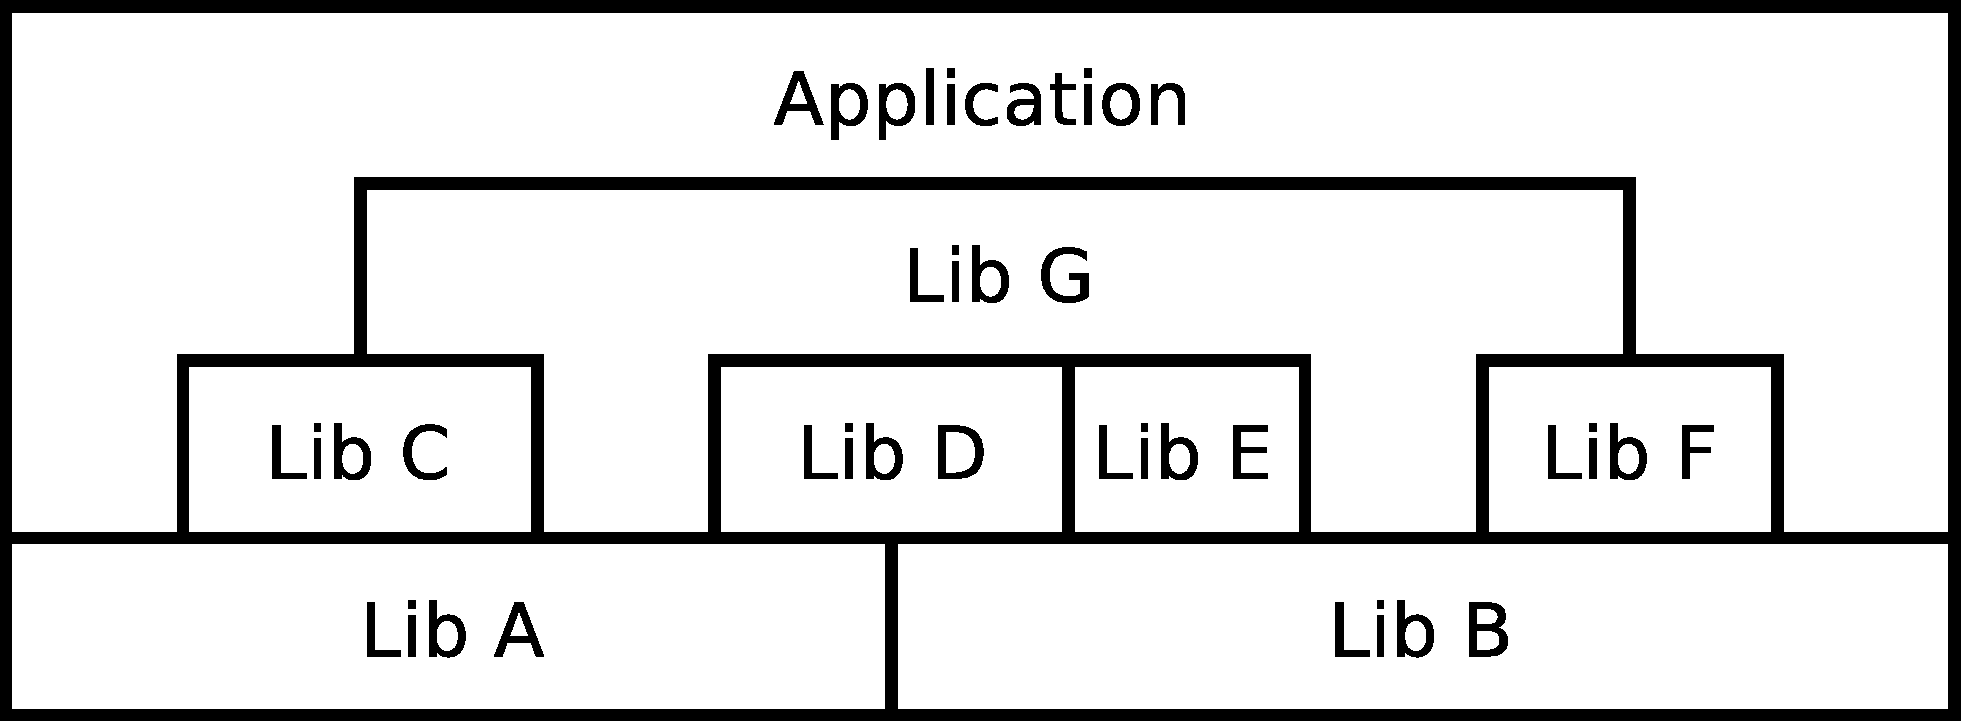
\includegraphics[scale=0.25]{images/dag-usual-representation.pdf}
%     \caption{A typical diagram of a software architecture, what is called a ``software stack''. It is actually a DAG: the Application can use (from left to right) Lib~A, Lib~C, Lib~G, Lib~F and Lib~B. Lib~D and Lib~E are internal libraries and cannot be used by the Application.} % FIXME: not good explanation for why it's a DAG. The Lib~A can be used by Lib~C, Lib~G, Lib~D and the Application.
%     \label{fig:dag-usual-representation}
%   \end{center}
% \end{figure}
%
% You may be familiar with a software architecture diagram like in Figure~\ref{fig:dag-usual-representation}, which is commonly called a ``software stack''. But it is actually a directed acyclic graph (DAG).

\end{document}
